\documentclass[12pt,a4paper]{article}
\usepackage[british]{babel}
\usepackage[a4paper,margin=1in]{geometry}
\usepackage{mathptmx}
\usepackage[round,authoryear]{natbib}
\usepackage{graphicx,booktabs,float,caption,enumitem,amsmath}
\usepackage{xurl}
\usepackage[hidelinks]{hyperref}
\graphicspath{{../project/results/figures/}{../Week2_Submission/figures/}{./}}
\setlength{\parskip}{5pt}
\setlength{\parindent}{0pt}
\captionsetup{font=small}
\newcommand{\pdash}{-}

\begin{document}

\begin{titlepage}
\centering
\vspace*{2cm}
{\LARGE\bfseries Determining the Role of Big Data Applications in Fraud Detection and Financial Security in Financial Institutions of Ireland\par}
\vspace{1.5cm}
{\Large Research Project Dissertation\par}
\vspace{1.5cm}
{\large Yashwanth\par}
\vspace{0.6cm}
MSc Research Practicum, Open Data Practice\par
National College of Ireland\par
Supervisor: Dr.\ Prasanth Nayak\par
\vfill
{\large December 2026\par}
\end{titlepage}

\begin{abstract}
Payment fraud in Ireland reached 160 million euro in 2024, and card payments accounted for most fraudulent transactions by volume \citep{cbi2025fraud}. Rule-based systems struggle with this volume and with changing fraud patterns, so banks are turning to big data applications and machine learning. This study compares Logistic Regression, Decision Tree and Random Forest for detecting card fraud on the public ULB credit card dataset of 284{,}807 European transactions, of which only 0.17\% are fraud.

I built one reproducible pipeline. It removes 1{,}081 duplicate rows before splitting the data, uses a single stratified 70/30 split, tunes each model with cross-validation on the training data, and fits scaling and SMOTE on the training data only. Because fraud is so rare, models are compared on precision, recall, F1, PR-AUC and the Matthews correlation coefficient rather than accuracy.

Random Forest was the best model. With class weights it reached a PR-AUC of 0.823 and an F1 of 0.818 (95\% confidence interval 0.766 to 0.869), with only 4 false alarms among 84{,}976 legitimate test transactions. Logistic Regression and Decision Tree with class weights produced many false alarms at the default threshold, with F1 of 0.10 and 0.57. Choosing the decision threshold on validation data raised their F1 to 0.78 and 0.74, and Random Forest's to 0.84. When the model was trained on earlier transactions and tested on later ones, Random Forest kept an F1 of 0.79 while the other two models fell sharply. The study also shows that keeping duplicate rows would have placed 456 test transactions in the training data. The results support using Random Forest with careful evaluation, and the discussion relates them to GDPR, PSD2 and the EU AI Act for Irish financial institutions.

\medskip
\textbf{Keywords:} big data, fraud detection, financial security, machine learning, Random Forest, Ireland
\end{abstract}

\newpage
\tableofcontents
\newpage

% ================================================================ 1
\section{Introduction}\label{sec:intro}

\subsection{Background}
Irish banking has moved quickly to online, mobile and instant payments. These services produce large volumes of transaction data every second, and they also give fraudsters more ways in. The Central Bank of Ireland reports that the value of fraudulent payments rose from 102 million euro in 2022 to 160 million euro in 2024, and the number of fraudulent transactions rose to about 815{,}000 in 2024, most of them card payments \citep{cbi2025fraud}.

Big data applications let banks store and process every transaction as it happens, and machine learning models can learn the patterns that separate fraud from normal spending. Distributed engines such as Apache Spark \citep{zaharia2016spark} make this possible at bank scale, while libraries such as scikit-learn \citep{pedregosa2011scikit} make the models themselves easy to build and test.

\subsection{Research problem}
Traditional fraud systems depend on fixed rules. Rules are easy to explain, but they have to be updated by hand, they miss new fraud patterns, and they often raise many false alarms. Machine learning can help, but card fraud is extremely rare, so a model that simply predicts ``not fraud'' for everything can look almost perfect on accuracy while catching nothing. Choosing the right model, the right way to handle imbalance and the right way to measure success is therefore a practical problem for Irish banks.

\subsection{Research gap}
Many studies compare machine learning models on card fraud data, but the reading in Section~\ref{sec:lit} shows several weaknesses. Most rely on accuracy, few report PR-AUC, few say whether SMOTE was applied before or after splitting the data, and none mention the duplicate rows in the most common benchmark. Very few studies connect the results to Irish or EU regulation. This study addresses these points with a careful comparison of Logistic Regression, Decision Tree and Random Forest.

\subsection{Aim, objectives and research questions}
\textbf{Aim.} To evaluate the role of big data applications in fraud detection and the improvement of financial security frameworks within financial institutions in Ireland.

\textbf{Objectives.}
\begin{enumerate}[nosep]
\item To identify the applications of big data in fraud detection and the improvement of financial security in financial institutions.
\item To examine the role of big data applications in improving regulatory standards and ethical considerations in financial security in Ireland.
\item To analyse the current challenges within financial institutions in Ireland for fraud detection.
\item To provide recommendations for implementing big data applications in fraud detection systems in Irish financial institutions.
\end{enumerate}

\textbf{Research questions.}
\begin{description}[nosep,leftmargin=1.2cm,labelwidth=1cm]
\item[RQ1] What are the applications of big data for fraud detection and the improvement of financial security in financial institutions, and how well do machine learning models perform on real card transactions?
\item[RQ2] What is the role of big data applications in strengthening regulatory standards and ethical considerations in the financial security of the financial industry in Ireland?
\item[RQ3] What are the current challenges faced by financial institutions in Ireland in detecting fraud and improving security mechanisms?
\end{description}

\subsection{Contribution}
The study contributes a reproducible pipeline that anyone can run with one command, a fair comparison of three models under three ways of handling imbalance, evidence on duplicate leakage and threshold choice that earlier studies do not report, and recommendations for Irish institutions grounded in these results.

\subsection{Structure}
Section~\ref{sec:lit} reviews the literature. Section~\ref{sec:method} describes the method, Section~\ref{sec:impl} the implementation and Section~\ref{sec:eval} the results. Section~\ref{sec:disc} discusses the findings against the research questions and Section~\ref{sec:concl} concludes.

% ================================================================ 2
\section{Literature Review}\label{sec:lit}

\subsection{Big data analytics in financial fraud detection}
\citet{jamil2025bigdata} studied fraud detection in the USA using Logistic Regression, Decision Tree and Random Forest on transaction data with demographic and location features. All models reached very high accuracy, so the authors compared errors instead; Random Forest gave the best balance, with 204 false positives against 594 for the Decision Tree. The paper discusses big data in general terms but does not test a big data platform. \citet{elumilade2025leveraging} review how financial data analytics supports fraud prevention through machine learning, anomaly detection and real-time monitoring, and they name data privacy and legacy systems as the main barriers.

\citet{gkegkas2025review} carried out a systematic review of 43 studies on financial statement fraud. They group methods into supervised machine learning, statistical anomaly detection, network analysis and real-time monitoring, and they identify class imbalance, poor interpretability and weak governance as the main challenges.

\subsection{Machine learning models for card and banking fraud}
\citet{salunke2025hybrid} compare Logistic Regression, Decision Tree and Random Forest on a public card fraud dataset and find that a hybrid of the three beats each model alone. \citet{albalawi2025enhancing} use the same ULB dataset as this study and test Logistic Regression, Decision Tree, Random Forest, XGBoost and a deep learning model with SMOTE. In their abstract Random Forest performs best, with an F1 of 0.8256 and a ROC-AUC of 0.9759, and they check their findings on PaySim. \citet{andrade2025smote} compare seven models on the ULB data after SMOTE with an 80/20 split. Random Forest has the best F1 (0.872, AUC 0.978), XGBoost is close (F1 0.837), and Logistic Regression reaches an F1 of only 0.110 despite high accuracy.

\citet{appavu2025ai} group cardholders by spending, build features over a sliding window of recent transactions and add a feedback loop for concept drift, training Decision Tree and Logistic Regression models for each group. \citet{preciado2025banking} test Random Forest, a neural network and Naive Bayes on about 565{,}000 bank transfers and find Random Forest the most reliable, with 95.79\% fraud detection accuracy. \citet{haider2024pca} apply scaling, PCA and SMOTE before six models and report about 96 to 97\% accuracy, but only accuracy. \citet{alrasheedi2025enhancing} compares seven models across three datasets; Random Forest reaches 0.97 accuracy on the imbalanced dataset with better fraud precision and recall.

\subsection{Class imbalance and evaluation}
Card fraud datasets are extremely imbalanced. SMOTE \citep{chawla2002smote} creates synthetic minority examples, and it appears in most of the studies above. \citet{ma2026leakage} are careful to keep the test set at the original class balance (85{,}443 transactions with 148 frauds). Their best tuned XGBoost reached a PR-AUC of 0.798 and a fraud F1 of 0.809, and they found that resampling is not always beneficial and must be judged on the real class distribution. \citet{baisholan2025review} review only studies that keep the original imbalance. They find that tree ensembles dominate, that most studies use a few public datasets, and that AUC-PR is used much less than it should be. \citet{saito2015precision} show why: on imbalanced data the precision-recall curve is more informative than the ROC curve.

\subsection{Regulation, trust and explainability}
\citet{horobets2025aml} discuss AI for anti-money laundering in European banks under the Sixth Anti-Money Laundering Directive and the AI Act, and conclude that aligning explainability, confidentiality, fairness and data security with what AI can deliver is still unresolved. \citet{bian2025review} list interpretability, class imbalance, drifting fraud patterns and restricted data access as open problems and suggest federated learning and GAN-based oversampling. \citet{khan2026fintech} surveyed 385 professionals in Pakistani FinTech and banking, who rated AI fraud detection and real-time monitoring as effective. In Ireland, GDPR \citep{gdpr2016} gives customers rights around automated decisions, PSD2 \citep{psd2015} requires strong customer authentication and transaction monitoring, and the EU AI Act \citep{euaiact2024} adds obligations for high-risk AI systems.

\subsection{Research niche}
Table~\ref{tab:lit} summarises the experimental studies. Across them, Random Forest is consistently strong, but results are often reported with accuracy, the timing of SMOTE is rarely stated, the ULB duplicates are never mentioned, and the Irish context is missing. This study fills that niche.

\begin{table}[H]
\centering\small
\caption{Experimental studies used for comparison.}\label{tab:lit}
\begin{tabular}{p{4.3cm}p{3.1cm}p{3.6cm}p{3.1cm}}
\toprule
Study & Data & Models & Main result \\
\midrule
\citet{albalawi2025enhancing} & ULB, PaySim & LR, DT, RF, XGBoost, DL & RF F1 0.826 \\
\citet{andrade2025smote} & ULB & Seven models with SMOTE & RF F1 0.872 \\
\citet{ma2026leakage} & ULB & Tuned XGBoost & PR-AUC 0.798 \\
\citet{preciado2025banking} & Bank transfers & RF, NN, NB & RF best \\
\citet{jamil2025bigdata} & US transactions & LR, DT, RF & RF fewest errors \\
\citet{salunke2025hybrid} & Card dataset & LR, DT, RF, hybrid & Hybrid best \\
\citet{alrasheedi2025enhancing} & Three datasets & Seven models & RF 0.97 accuracy \\
\bottomrule
\end{tabular}
\end{table}

% ================================================================ 3
\section{Research Methodology}\label{sec:method}

\subsection{Research approach}
The study follows a quantitative experimental design. The same data, split and evaluation are used for every model, so that differences come from the models and not from the set-up.

\subsection{Dataset}
The ULB credit card dataset \citep{kaggle2018ulb, dalpozzolo2015calibrating} contains 284{,}807 transactions made by European cardholders over two days in September 2013, with 492 frauds (0.173\%). To protect cardholders, the owners replaced the original features with 28 PCA components, V1 to V28; only Time (seconds from the first transaction) and Amount keep their meaning. The dataset was chosen over IEEE-CIS, PaySim \citep{lopezrojas2016paysim} and the Bank Account Fraud suite \citep{jesus2022turning} because it contains real European card payments, has an open licence, and is used by most of the comparison studies. Figure~\ref{fig:class} shows the imbalance.

\begin{figure}[H]
\centering
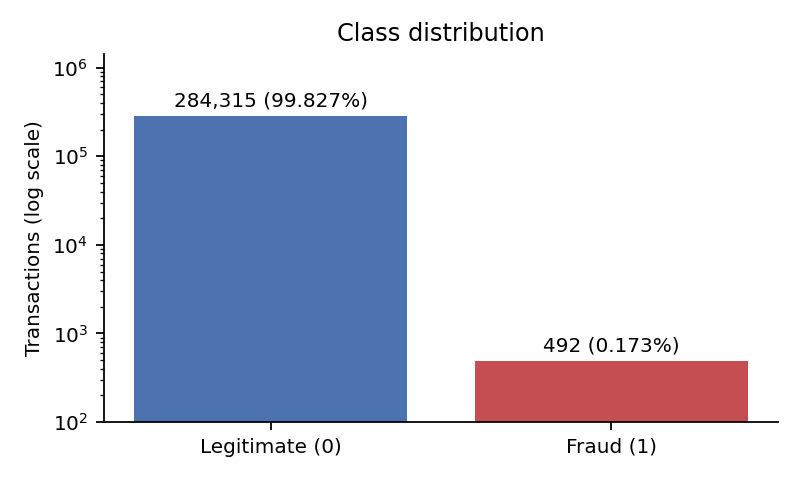
\includegraphics[width=0.55\linewidth]{w2_class_balance}
\caption{Legitimate and fraud transactions (log scale).}\label{fig:class}
\end{figure}

\subsection{Data preparation}
The data has no missing values, but 1{,}081 rows are exact copies of other rows, 19 of them fraud. These were removed before splitting, leaving 283{,}726 transactions with 473 frauds. An hour-of-day feature was derived from Time. The data was then split once into 70\% training and 30\% test data, stratified by class, with a fixed random seed of 42. This gives 198{,}608 training rows with 331 frauds and 85{,}118 test rows with 142 frauds. Amount, Time and Hour are standardised; the scaler is fitted on the training data only.

\subsection{Models}
\begin{itemize}[nosep]
\item \textbf{Logistic Regression}: a linear model that gives a probability of fraud; a simple and transparent baseline.
\item \textbf{Decision Tree} \citep{breiman1984classification}: a set of if-then rules that is easy to explain.
\item \textbf{Random Forest} \citep{breiman2001random}: an average of 200 decision trees trained on random samples of rows and features, which reduces the variance of a single tree.
\end{itemize}

\subsection{Handling imbalance}
Three strategies were compared for every model: no resampling, class weights that give fraud cases more weight during training, and SMOTE \citep{chawla2002smote}. SMOTE is placed inside the model pipeline, so it only ever sees the training data of each fold; synthetic fraud cases never reach the test set.

\subsection{Tuning and evaluation}
Each model was tuned with stratified 3-fold cross-validation on the training data, using PR-AUC as the score. The tuned models were then evaluated once on the test set with precision, recall, F1, PR-AUC, ROC-AUC, the Matthews correlation coefficient (MCC) and accuracy. A 95\% bootstrap confidence interval was computed for F1, and McNemar's test \citep{dietterich1998approximate} was used to check whether the best model differs significantly from the others. The decision threshold was chosen on a validation slice of the training data (25\%), never on the test data.

\subsection{Robustness and explainability}
Four further checks were run: the effect of keeping duplicates, a time-based split (train on the first 70\% of the time period, test on the rest), an ablation of the hour feature, and training time as the data grows. For explanation, Random Forest impurity and permutation importance, Logistic Regression coefficients and SHAP values \citep{lundberg2017unified} were computed.

\subsection{Ethics}
The data is anonymised and contains no personal identifiers. It is used for research under its licence and is not redistributed. Because the data comes from European cardholders in 2013, results are presented as evidence about methods, and the Irish recommendations draw on the literature and Central Bank statistics.

% ================================================================ 4
\section{Implementation}\label{sec:impl}
The whole experiment is one Python script, \texttt{src/pipeline.py}, built on pandas, scikit-learn \citep{pedregosa2011scikit}, imbalanced-learn and SHAP. Each model is wrapped in a pipeline of scaling, optional SMOTE and the classifier, so that every step that learns from data is fitted on training data only. A check in the script stops the run if any test row also appears in the training data. The script writes every table to \texttt{results/tables} and every figure to \texttt{results/figures}; the numbers in this report come from those files. The full run takes about six minutes on a laptop. Table~\ref{tab:tune} shows the tuned settings.

\begin{table}[H]
\centering\small
\caption{Tuned settings and cross-validated PR-AUC on the training data.}\label{tab:tune}
\begin{tabular}{llc}
\toprule
Model & Selected settings & CV PR-AUC (sd) \\
\midrule
Logistic Regression & C = 1.0 & 0.746 (0.026) \\
Decision Tree & max depth 20, min samples per leaf 10 & 0.738 (0.017) \\
Random Forest & 200 trees, no depth limit, min samples per leaf 1 & 0.840 (0.007) \\
\bottomrule
\end{tabular}
\end{table}

% ================================================================ 5
\section{Evaluation}\label{sec:eval}

\subsection{Main results}
Table~\ref{tab:main} shows the three models with class weights, as planned in the proposal, at the default threshold of 0.5.

\begin{table}[H]
\centering\small
\caption{Test results with class weights and threshold 0.5 (85{,}118 test transactions, 142 frauds).}\label{tab:main}
\resizebox{\linewidth}{!}{\begin{tabular}{lccccccc}
\toprule
Model & Precision & Recall & F1 (95\% CI) & MCC & PR-AUC & ROC-AUC & False alarms \\
\midrule
Random Forest & 0.962 & 0.711 & 0.818 (0.766 to 0.869) & 0.827 & 0.823 & 0.945 & 4 \\
Decision Tree & 0.461 & 0.746 & 0.570 (0.509 to 0.626) & 0.586 & 0.704 & 0.873 & 124 \\
Logistic Regression & 0.053 & 0.887 & 0.100 (0.083 to 0.117) & 0.213 & 0.687 & 0.970 & 2{,}264 \\
\bottomrule
\end{tabular}}
\end{table}

Random Forest is clearly the best model. It catches 101 of the 142 frauds while raising only 4 false alarms. Logistic Regression catches the most frauds (126) but raises 2{,}264 false alarms, and every one of them would need to be checked by an analyst. Its accuracy is still 97.3\%, which shows how misleading accuracy is on this data. McNemar's test confirms that Random Forest differs significantly from both other models ($p<0.001$). Figure~\ref{fig:roc} shows the ROC and precision-recall curves; Logistic Regression has the highest ROC-AUC but a much lower PR-AUC, which is the pattern described by \citet{saito2015precision}.

\begin{figure}[H]
\centering
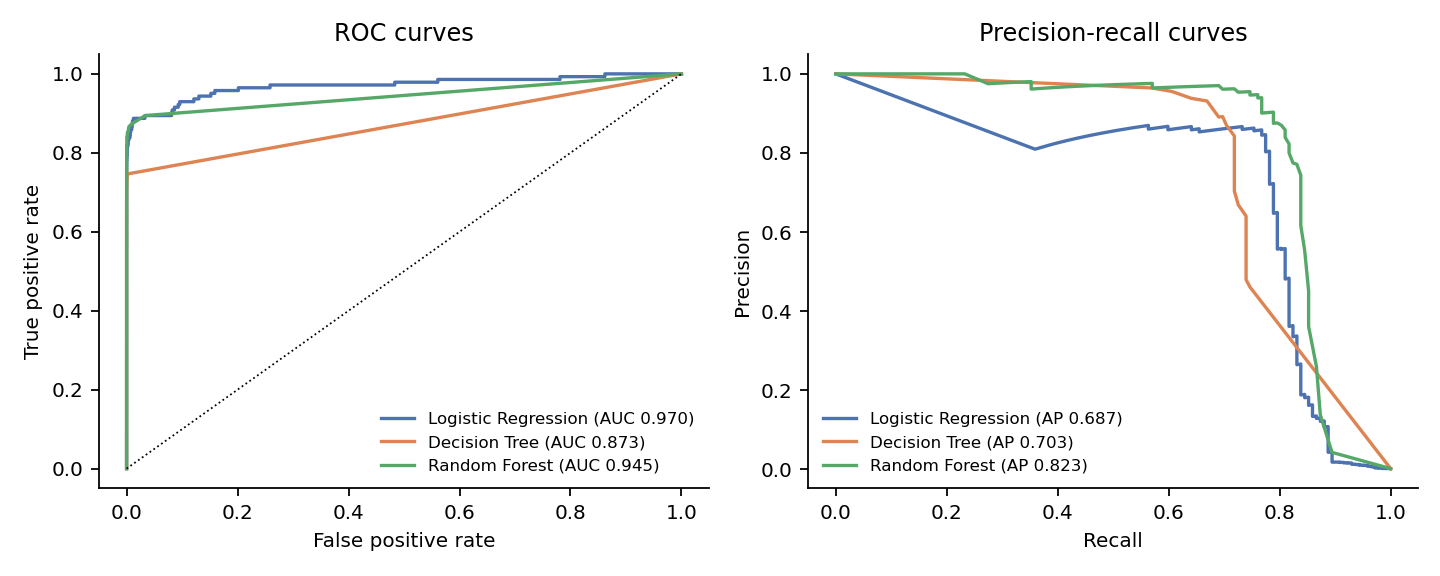
\includegraphics[width=\linewidth]{roc_pr_curves}
\caption{ROC curves (left) and precision-recall curves (right) on the test set.}\label{fig:roc}
\end{figure}

\begin{figure}[H]
\centering
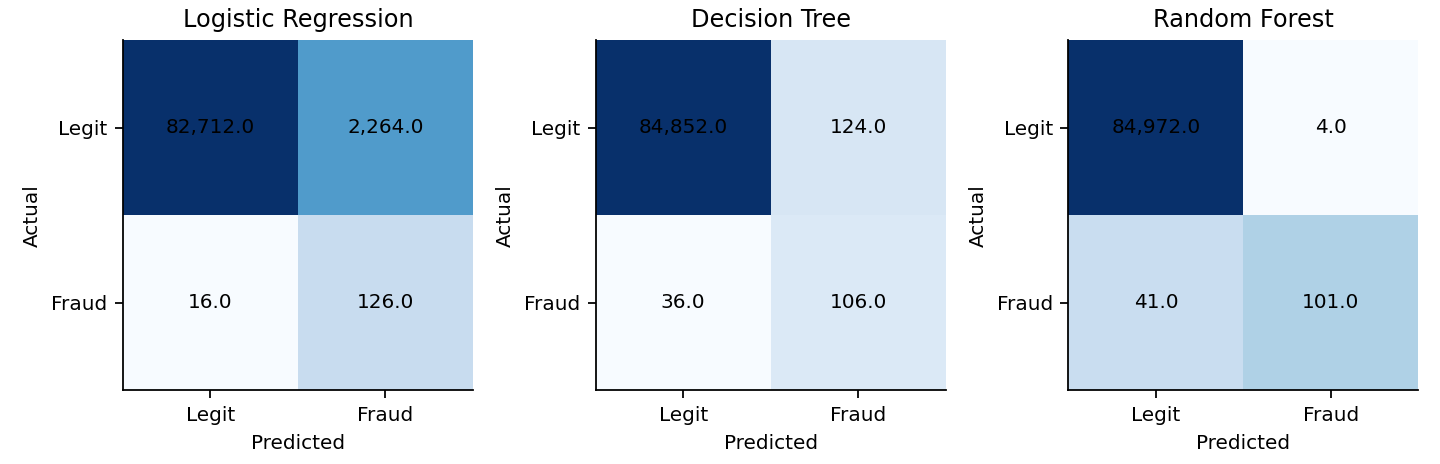
\includegraphics[width=\linewidth]{confusion_matrices}
\caption{Confusion matrices with class weights and threshold 0.5.}\label{fig:cm}
\end{figure}

\subsection{Effect of imbalance handling}
Table~\ref{tab:strat} compares the three strategies. For Random Forest the choice matters little: F1 is between 0.818 and 0.838 and PR-AUC between 0.804 and 0.823. For Logistic Regression and Decision Tree, class weights and SMOTE make the default threshold far too low, so precision collapses. Decision Tree with SMOTE is the worst case, with a PR-AUC of only 0.382. This supports the warning of \citet{ma2026leakage} that resampling is not always helpful.

\begin{table}[H]
\centering\small
\caption{F1 and PR-AUC on the test set for each imbalance strategy.}\label{tab:strat}
\begin{tabular}{lcccccc}
\toprule
& \multicolumn{2}{c}{No resampling} & \multicolumn{2}{c}{Class weights} & \multicolumn{2}{c}{SMOTE} \\
Model & F1 & PR-AUC & F1 & PR-AUC & F1 & PR-AUC \\
\midrule
Logistic Regression & 0.683 & 0.704 & 0.100 & 0.687 & 0.095 & 0.693 \\
Decision Tree & 0.786 & 0.698 & 0.570 & 0.704 & 0.386 & 0.382 \\
Random Forest & 0.829 & 0.804 & 0.818 & 0.823 & 0.838 & 0.822 \\
\bottomrule
\end{tabular}
\end{table}

\begin{figure}[H]
\centering
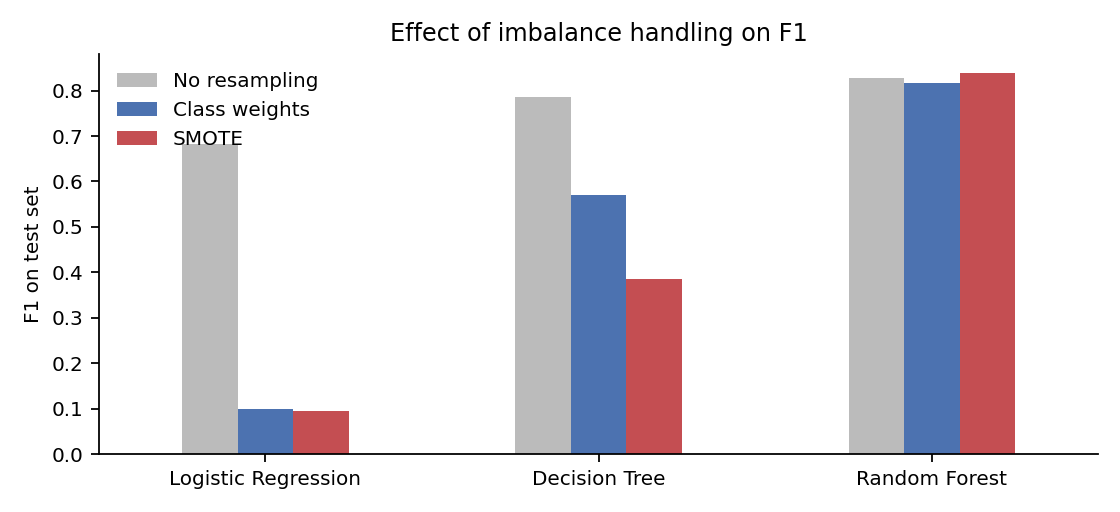
\includegraphics[width=0.75\linewidth]{imbalance_f1}
\caption{F1 on the test set by imbalance strategy.}\label{fig:imb}
\end{figure}

\subsection{Choosing the decision threshold}
Table~\ref{tab:thr} shows what happens when the threshold is chosen on validation data instead of fixing it at 0.5. Logistic Regression rises from an F1 of 0.100 to 0.785 and Decision Tree from 0.570 to 0.741, because the new thresholds remove most false alarms. Random Forest improves from 0.818 to 0.844 with a threshold of 0.34, catching 108 frauds with 6 false alarms. Figure~\ref{fig:thr} shows the trade-off for Random Forest.

\begin{table}[H]
\centering\small
\caption{Test results at the threshold chosen on validation data (class weights).}\label{tab:thr}
\begin{tabular}{lccccc}
\toprule
Model & F1 at 0.5 & F1 at tuned threshold & Precision & Recall & False alarms \\
\midrule
Random Forest & 0.818 & 0.844 & 0.947 & 0.761 & 6 \\
Logistic Regression & 0.100 & 0.785 & 0.864 & 0.718 & 16 \\
Decision Tree & 0.570 & 0.741 & 0.956 & 0.606 & 4 \\
\bottomrule
\end{tabular}
\end{table}

\begin{figure}[H]
\centering
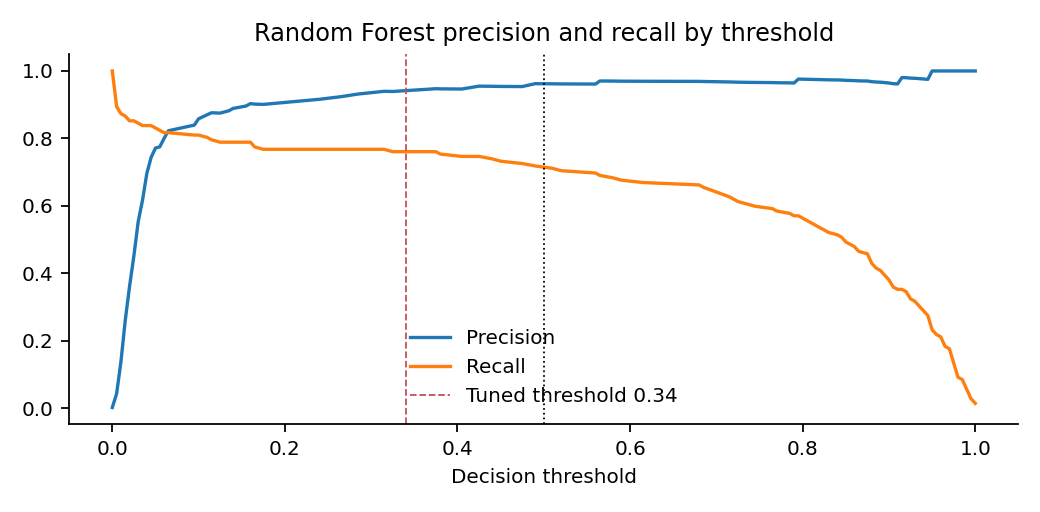
\includegraphics[width=0.75\linewidth]{threshold_tradeoff}
\caption{Random Forest precision and recall at different thresholds.}\label{fig:thr}
\end{figure}

\subsection{Robustness}
\textbf{Duplicates.} If the duplicates are not removed, 456 of the test rows also appear in the training data, 7 of them fraud. A model would be rewarded for remembering them, so earlier studies that do not remove duplicates may overstate their results slightly.

\textbf{Time-based split.} When the models are trained on the first 70\% of the two days and tested on the rest, Random Forest keeps an F1 of 0.791 with no false alarms and a recall of 0.654. Decision Tree falls to 0.414 and Logistic Regression to 0.081, so Random Forest is also the most stable model over time.

\textbf{Hour feature.} Adding the hour of day did not change Random Forest's F1 (0.818 with and without it), so the night-time pattern seen in the data exploration is already captured by the other features.

\textbf{Training time.} Random Forest took 0.42 seconds on 19{,}860 rows and 16.4 seconds on the full 198{,}608 training rows (Figure~\ref{fig:scale}). Scoring takes well under a millisecond per transaction, which is fast enough for real-time use.

\begin{figure}[H]
\centering
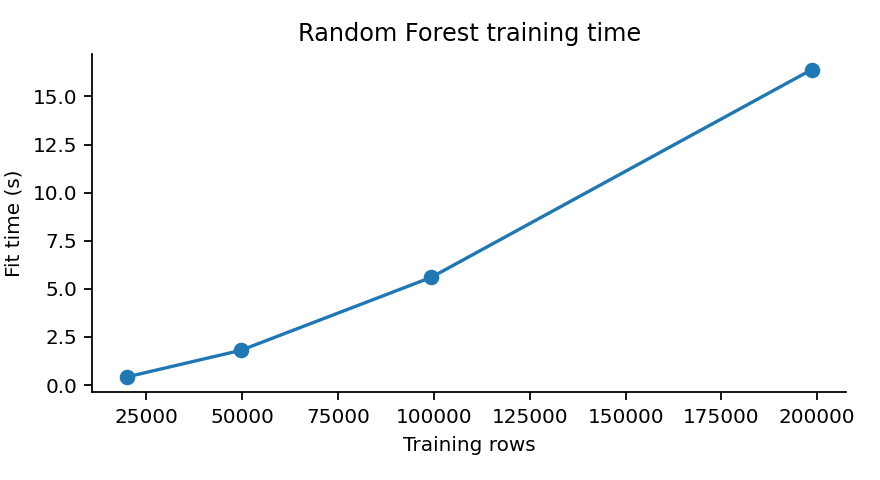
\includegraphics[width=0.6\linewidth]{scalability}
\caption{Random Forest training time as the training set grows.}\label{fig:scale}
\end{figure}

\subsection{Explainability}
Permutation importance (Figure~\ref{fig:imp}) shows that shuffling V4 causes the largest drop in PR-AUC (0.087), followed by V9, V12, V3 and V14. The impurity importance of the forest ranks V14 highest, followed by V4, V10 and V12. The SHAP summary (Figure~\ref{fig:shap}) confirms that low values of V14, V12 and V10 and high values of V4 push predictions towards fraud. Because these are PCA components, a bank cannot tell a customer which real behaviour caused the alert, which is a limitation discussed below.

\begin{figure}[H]
\centering
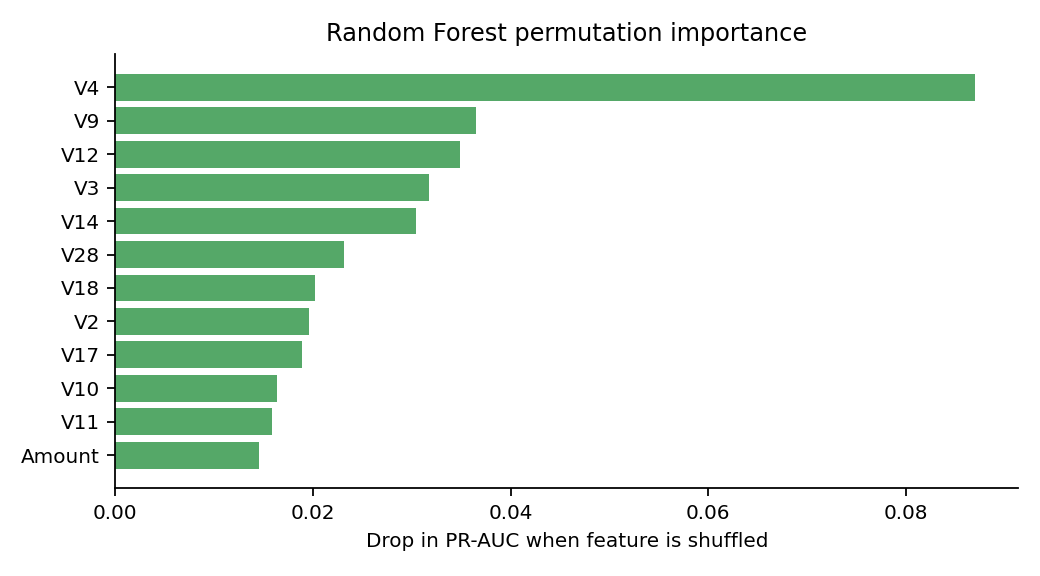
\includegraphics[width=0.75\linewidth]{feature_importance}
\caption{Random Forest permutation importance (drop in PR-AUC).}\label{fig:imp}
\end{figure}

\begin{figure}[H]
\centering
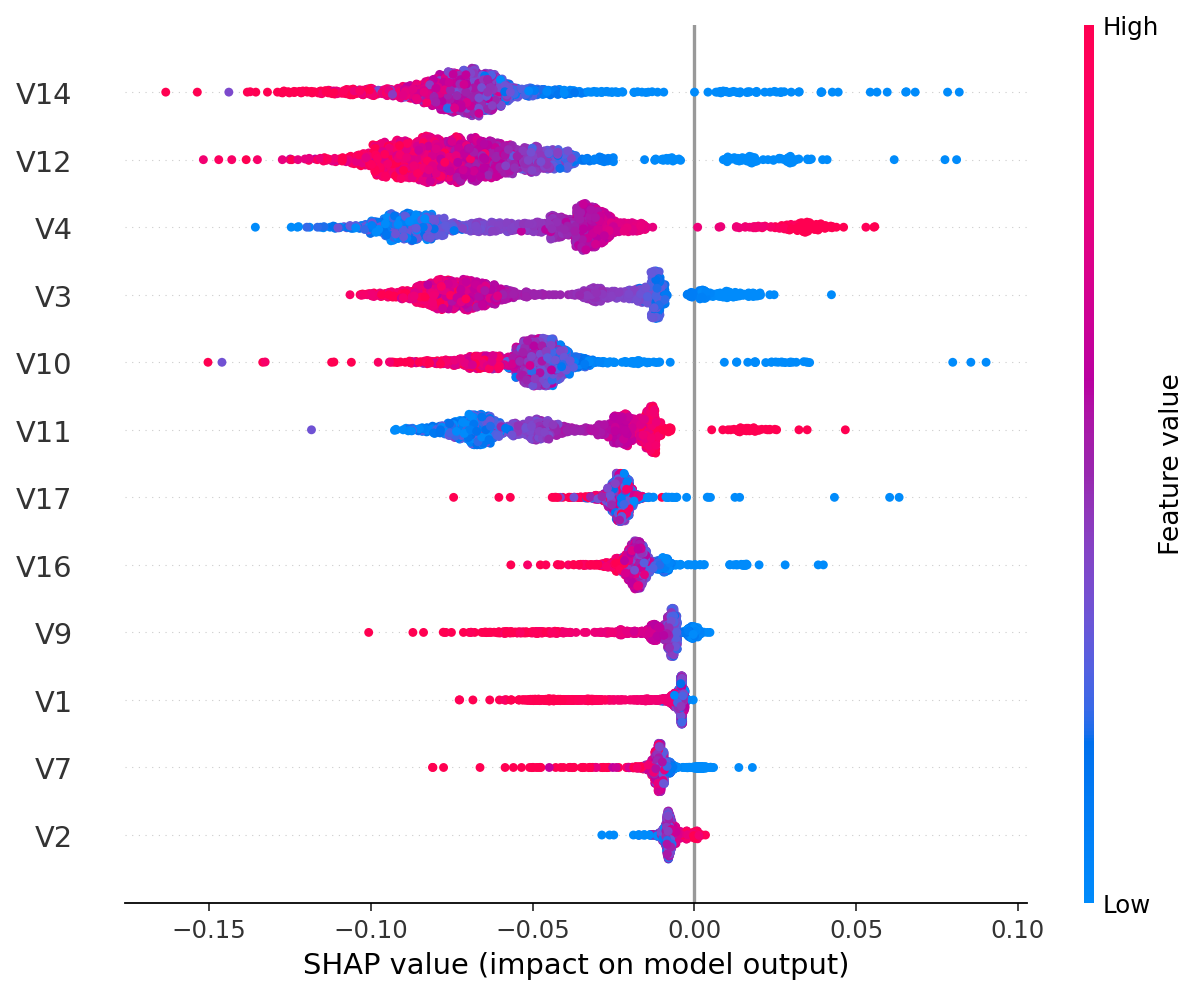
\includegraphics[width=0.7\linewidth]{shap_summary}
\caption{SHAP summary for Random Forest on 1{,}500 test transactions.}\label{fig:shap}
\end{figure}

% ================================================================ 6
\section{Discussion}\label{sec:disc}

\subsection{RQ1: applications and model performance}
Big data applications help at two points: processing every transaction in real time, and learning fraud patterns from large histories. The results show that Random Forest is the best of the three models on real card data, which matches \citet{albalawi2025enhancing}, \citet{andrade2025smote} and \citet{preciado2025banking}. Its F1 of 0.818 to 0.844 is close to the 0.826 and 0.872 reported on the same dataset by those studies. The more important finding is how much the set-up matters. Logistic Regression looked useless at the default threshold (F1 0.100) but reasonable after the threshold was chosen on validation data (0.785). Studies that report a single number without saying how the threshold or resampling was chosen are therefore hard to compare.

\subsection{RQ2: regulation and ethics}
Irish institutions work under GDPR, PSD2 and, increasingly, the EU AI Act. A fraud model that blocks payments affects customers directly, so banks must be able to explain decisions and show that models are tested fairly. Three results matter here. First, the low false alarm rate of Random Forest (4 to 6 in about 85{,}000 legitimate payments) limits the number of customers wrongly blocked. Second, SHAP and permutation importance show which inputs drive each decision, which supports the explanation duties discussed by \citet{horobets2025aml}. Third, the PCA features show the limit of explanation: on anonymised data, the model can be explained only in terms of components, not real behaviour. A bank using its own data would need interpretable features to meet GDPR expectations.

\subsection{RQ3: challenges}
The experiments illustrate four challenges that match the literature. Fraud is extremely rare, so accuracy is misleading and the threshold has to be chosen carefully. Resampling can harm simpler models, as \citet{ma2026leakage} also found. Data quality problems such as duplicates can leak test data into training. And fraud patterns change over time: even the best model lost some recall on the later time period. Irish institutions also face legacy systems and privacy barriers when sharing data \citep{elumilade2025leveraging, bian2025review}.

\subsection{Recommendations for Irish financial institutions}
\begin{enumerate}[nosep]
\item Use an ensemble model such as Random Forest as the core fraud scorer, alongside existing rules.
\item Judge models on precision, recall, F1 and PR-AUC, and never on accuracy alone.
\item Choose the alert threshold on validation data that reflects the real fraud rate and the cost of reviewing alerts.
\item Remove duplicates and fit every preprocessing step on training data only, to avoid leakage.
\item Retrain and test models regularly on the most recent period to detect drift.
\item Keep an explanation for every alert (for example SHAP values) to support GDPR and AI Act duties.
\end{enumerate}

\subsection{Limitations}
The dataset covers only two days in 2013, is not Irish, and uses PCA features, so the absolute scores may not transfer to a current Irish bank. Only three model families were compared, and the big data aspect was tested through training time on a single machine rather than a distributed platform.

% ================================================================ 7
\section{Conclusion and Future Work}\label{sec:concl}
This study compared Logistic Regression, Decision Tree and Random Forest for card fraud detection with a careful, reproducible pipeline. Random Forest was the best and most stable model, with a PR-AUC of 0.823 and an F1 of 0.818, rising to 0.844 when the threshold was chosen on validation data, and with very few false alarms. The study also showed that the evaluation set-up can change conclusions as much as the model choice: default thresholds, resampling and duplicates all affect the results. For Irish financial institutions, big data applications are most useful when combined with honest evaluation, regular retraining and clear explanations. Future work should test the pipeline on recent Irish or European transaction data with interpretable features, compare gradient boosting models, and run the pipeline on a distributed platform such as Spark.

% ================================================================ appendix
\section*{Reproducibility}
\addcontentsline{toc}{section}{Reproducibility}
Download the dataset with \texttt{kaggle datasets download -d mlg-ulb/creditcardfraud} into \texttt{project/data}, install \texttt{project/requirements.txt}, and run \texttt{python src/pipeline.py} from the \texttt{project} folder. All tables and figures are regenerated in \texttt{project/results}.

\section*{Project Plan}
\addcontentsline{toc}{section}{Project Plan}
Figure~\ref{fig:gantt} shows the twelve-week plan from the proposal. All phases were completed.

\begin{figure}[H]
\centering
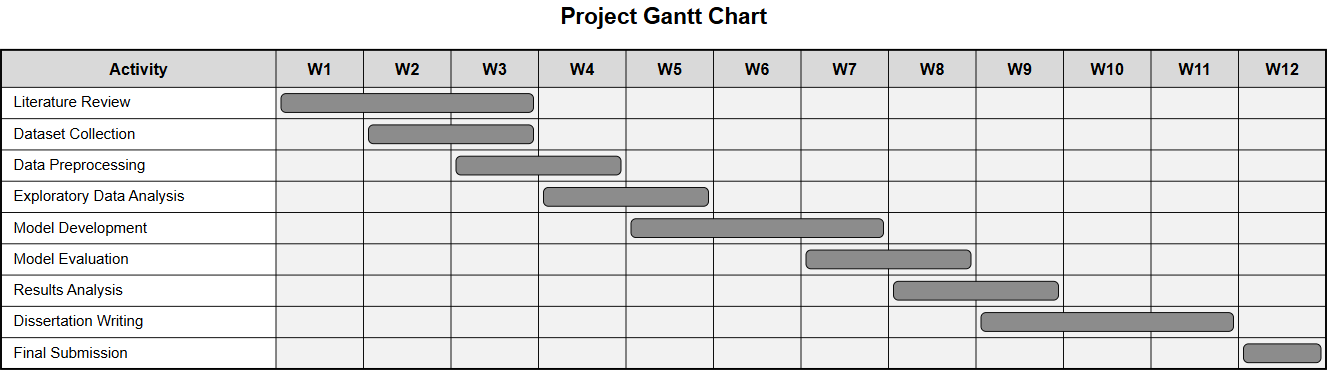
\includegraphics[width=\linewidth]{gantt_chart}
\caption{Project Gantt chart.}\label{fig:gantt}
\end{figure}

\newpage
\bibliographystyle{plainnat}
\bibliography{refs}

\end{document}
